\documentclass[11pt,a4paper]{article}

\usepackage[utf8]{inputenc}
\usepackage[T1]{fontenc}
\usepackage{lmodern}
\usepackage{amsmath,amssymb,amsthm}
\usepackage{tikz}
\usetikzlibrary{automata,positioning,arrows.meta}
\usepackage{listings}
\usepackage{xcolor}
\usepackage{hyperref}
\usepackage{geometry}
\usepackage{booktabs}
\usepackage{enumitem}
\usepackage{parskip}

\geometry{margin=1.2in}
\setlength{\parindent}{0pt}

\hypersetup{
    colorlinks=true,
    linkcolor=blue!60!black,
    urlcolor=blue!60!black,
    citecolor=blue!60!black
}

\definecolor{codebg}{RGB}{248,248,248}
\definecolor{codegreen}{RGB}{40,160,80}
\definecolor{codegray}{RGB}{128,128,128}
\definecolor{codeblue}{RGB}{40,80,160}
\definecolor{codered}{RGB}{180,40,40}

\lstdefinestyle{gostyle}{
    backgroundcolor=\color{codebg},
    commentstyle=\color{codegreen},
    keywordstyle=\color{codeblue}\bfseries,
    numberstyle=\tiny\color{codegray},
    stringstyle=\color{codered},
    basicstyle=\ttfamily\small,
    breakatwhitespace=false,
    breaklines=true,
    captionpos=b,
    keepspaces=true,
    numbers=left,
    numbersep=8pt,
    showspaces=false,
    showstringspaces=false,
    showtabs=false,
    tabsize=4,
    frame=single,
    framerule=0.5pt,
    rulecolor=\color{codegray!50}
}

\lstset{style=gostyle}

\newtheorem{definition}{Definition}

\title{\textbf{When Regex Isn't Fast Enough} \\[0.5em]
\large Building a Custom DFA for High-Traffic Validation}
\author{Jose Sitanggang \\[0.3em]
\small \url{https://josestg.com} \\
\small \url{https://github.com/josestg} \\
\small \href{mailto:me@josestg.com}{me@josestg.com}}
\date{\today}

\begin{document}

\maketitle

\begin{abstract}
Regular expressions are great for most use cases. But in high-traffic services where every microsecond counts, sometimes you need more control. This paper documents one such case: building a Deterministic Finite Automaton by hand for string validation. Using identifier validation as a running example, we walk through the process of formalizing the problem as a regular language, designing the states and transitions, and implementing the result in Go. The final implementation runs in \(O(n)\) time, uses constant memory, and makes zero heap allocations. This is not an argument against regex. It is an argument for learning the fundamentals. When you understand what regex engines do under the hood, you gain the option to build something custom when the situation calls for it.
\end{abstract}


% =============================================================================
\section{Introduction}
% =============================================================================

String validation is everywhere. Parsing configuration files, validating user input, processing API requests. You often need to check if a string matches a specific pattern.

The usual solution is a regular expression. Quick to write, gets the job done. But regex engines can have unpredictable performance, especially those with backtracking. For hot paths where validation runs on every request, this unpredictability becomes a problem.

\subsection{Background}

At work, I maintain a high-traffic service where latency matters. Every microsecond counts. String validation often sits in the hot path. Code that executes on every request, sometimes multiple times.

The example in this paper is not the exact problem I solved in production. For privacy reasons, I simplified and adapted it. But the technique and the underlying concepts are the same. The real problem involved a different alphabet and different constraints, yet the approach translated directly: formalize the language, construct a DFA, implement it with a precomputed transition table.

\subsection{Why Not Just Use Regex?}

I could have used a regular expression and moved on. For most use cases, that would be the right call. Regex is well-tested, readable, and good enough for the majority of applications.

\textbf{But ``good enough'' is not always good enough}. When you need predictable performance, general-purpose tools start to show their limits. They are designed to handle any pattern you throw at them. That flexibility comes with overhead.

This is where fundamentals pay off. Understanding automata theory, something many of us learned in university and promptly forgot, gives you the \textbf{ability to build custom solutions for specific problems}. You are not limited to what libraries provide. You can design exactly what you need.

The point of this paper is not to convince you to replace every regex with a hand-rolled DFA. That would be overkill. The point is to show that knowing the fundamentals opens doors. When you hit a performance wall, you have options beyond ``try a different library.''

\subsection{The Plan}

We will go through the entire process: defining the problem formally, constructing the automaton step by step, and implementing it in Go. The result is a validator that runs in linear time, uses constant memory, and makes zero heap allocations.

% =============================================================================
\section{A Brief Refresher on Automata Theory}
% =============================================================================

Before diving into the problem, let me give a quick refresher on automata theory. If you remember this from your university courses, feel free to skip ahead.

\subsection{Automata}

An automaton is a mathematical model of computation. Think of it as an abstract machine that reads input one symbol at a time and transitions between states based on what it reads. When the input is exhausted, the machine either accepts or rejects the input depending on which state it ends up in.

The simplest form is a finite automaton. It has a finite number of states, a starting state, a set of accepting states, and transition rules that say ``if you are in state X and you read symbol Y, go to state Z.'' That is the entire model. No memory, no stack, no variables. Just states and transitions.

Despite this simplicity, finite automata are surprisingly powerful. They can recognize exactly the class of languages we call regular languages.

\subsection{Regex is a Language for Building Machines}

Here is a useful way to think about regular expressions: they are a specification language for finite automata.

When you write a regex like \verb|[a-z]+@[a-z]+\.[a-z]+|, you are not writing code that executes directly. You are describing a pattern. The regex engine reads this description and builds a machine that can recognize strings matching that pattern.

This is why regex feels declarative rather than imperative. You say what you want to match, not how to match it. The ``how'' is handled by converting your specification into an automaton.

Understanding this connection changes how you think about regex. A complex regex is not just a cryptic string of symbols. It is a program that compiles into a state machine. And if you understand state machines, you can build them directly when you need more control.

\subsection{NFA and DFA}

There are two flavors of finite automata.

A Nondeterministic Finite Automaton (NFA) allows flexibility in its transitions. From a given state, reading a symbol might lead to multiple possible next states. The NFA also allows \(\varepsilon\)-transitions, which are transitions that happen without consuming any input. When processing a string, an NFA is said to accept if there exists some path through these choices that leads to an accepting state.

A Deterministic Finite Automaton (DFA) is more restrictive. From each state, each symbol leads to exactly one next state. The path through the machine is completely determined by the input.

NFAs are easier to construct. When you convert a regex to an automaton, the natural result is an NFA. The union operator (\verb+|+) becomes a branch with multiple outgoing transitions. The Kleene star (\verb|*|) becomes a loop with \(\varepsilon\)-transitions.

DFAs are easier to execute. At each step, you look at the current state and the current input symbol, do one table lookup, and move to the next state. No backtracking, no exploring multiple paths. This is why DFAs give predictable \(O(n)\) performance.

\subsection{Converting NFA to DFA}

Every NFA can be converted to an equivalent DFA. This is called the subset construction, and it works by treating sets of NFA states as single DFA states.

The intuition is this: an NFA can be in multiple states simultaneously (because of nondeterminism). So we define a DFA state as a set of NFA states. The DFA simulates the NFA by tracking all possible states the NFA could be in after reading each symbol.

The process works like this. Start with the set containing just the NFA start state (plus any states reachable via \(\varepsilon\)-transitions). This becomes the DFA start state. For each DFA state (which is a set of NFA states) and each input symbol, compute where the NFA could go from any of those states. That set of destination states becomes a DFA state. Repeat until no new DFA states are created. A DFA state is accepting if it contains any accepting NFA state.

In the worst case, an NFA with \(n\) states can produce a DFA with \(2^n\) states. In practice, for most patterns, the blowup is much smaller.

\subsection{What Regex Engines Actually Do}

When a regex engine runs your pattern, it has choices. It can interpret the NFA directly, exploring paths and backtracking when needed. Or it can convert to a DFA first and then run the DFA.

Backtracking engines (like those in Perl, Python, and JavaScript) interpret the NFA. They are flexible and support features like backreferences, but they can have exponential worst-case time on pathological inputs.

DFA-based engines (like RE2, which Go uses) convert to a DFA. They guarantee linear time but cannot support some features that require memory, like backreferences.

When you write a DFA by hand, you skip all this machinery. You design the states yourself, define the transitions, and implement a tight loop that does nothing but table lookups. No regex parsing, no NFA construction, no subset construction at runtime. Just your specific automaton, exactly as you designed it.

% =============================================================================
\section{The Problem}
% =============================================================================

We want to validate identifiers with the following rules. The alphabet consists of letters (\texttt{a-z}, \texttt{A-Z}), digits (\texttt{0-9}), underscore (\texttt{\_}), and hyphen (\texttt{-}). The first character cannot be a digit. If the identifier starts with a symbol (\texttt{\_} or \texttt{-}), it must be followed by at least one letter or digit. Consecutive symbols are not allowed. The identifier cannot end with a hyphen.

Here are some examples:

\begin{table}[h]
\centering
\begin{tabular}{ll}
\toprule
\textbf{Valid} & \textbf{Invalid} \\
\midrule
\texttt{myVar} & \texttt{123abc} (starts with digit) \\
\texttt{\_private} & \texttt{\_} (symbol alone) \\
\texttt{kebab-case} & \texttt{a\_\_b} (consecutive symbols) \\
\texttt{snake\_case\_} & \texttt{test-} (hyphen suffix) \\
\texttt{-flag} & \texttt{--verbose} (consecutive symbols) \\
\bottomrule
\end{tabular}
\end{table}

% =============================================================================
\section{Formalizing the Language}
% =============================================================================

Before building an automaton, we need to describe our language formally. This gives us a precise specification to work from.

\subsection{Defining the Character Sets}

Let us define the character sets:

\begin{align*}
L &= \{a, b, \ldots, z, A, B, \ldots, Z\} && \text{letters} \\
D &= \{0, 1, \ldots, 9\} && \text{digits} \\
S &= \{\_, -\} && \text{symbols}
\end{align*}

The full alphabet is \(\Sigma = L \cup D \cup S\).

\subsection{The Pattern}

Our language can be split into two cases based on the first character.

If the string starts with a letter, we can have any sequence of alphanumerics after it, optionally separated by single symbols. The string can end with an underscore but not a hyphen.

If the string starts with a symbol, that symbol must be followed by at least one alphanumeric character. After that, the rules are the same.

Combining both cases:

\[
\Big( L \,|\, S(L \cup D) \Big) (L \cup D)^* \Big( S(L \cup D)^+ \Big)^* (\_)?
\]

In standard regex notation:

\begin{verbatim}
    ^([a-zA-Z]|[_-][a-zA-Z0-9])[a-zA-Z0-9]*([_-][a-zA-Z0-9]+)*_?$
\end{verbatim}

% =============================================================================
\section{Designing the Automaton}
% =============================================================================

Now we translate this language into a finite automaton. The standard approach is to build an NFA from the regex, then convert it to a DFA using the subset construction. Let us walk through this process.

\subsection{The Textbook Approach}

There is a mechanical procedure called Thompson's construction that converts any regex to an NFA. You build small NFAs for each primitive (single characters, empty string) and combine them using rules for concatenation, union, and Kleene star.

For our regex:
\[
\Big( L \,|\, S(L \cup D) \Big) (L \cup D)^* \Big( S(L \cup D)^+ \Big)^* (\_)?
\]

Following Thompson's construction would give us an NFA with many states and \(\varepsilon\)-transitions. The union \(L \,|\, S(L \cup D)\) would branch into two paths. The Kleene stars would create loops with \(\varepsilon\)-transitions back to earlier states.

But I want to show you a different approach. Instead of mechanically applying Thompson's construction and then running subset construction, we can think directly about what information the automaton needs to track. This often produces a simpler DFA without going through the NFA intermediate step.

\subsection{A Practical Way: Think About What to Remember}

What does the automaton need to remember as it reads characters?

It needs to know if it has just started, because different characters are valid at the start versus in the middle. It needs to know if it just read a symbol, because consecutive symbols are forbidden. It needs to know if it started with a symbol and has not yet seen an alphanumeric, because a symbol alone is invalid. And it needs to distinguish underscore from hyphen at the end, because hyphen suffixes are rejected while underscore suffixes are allowed.

Each of these ``things to remember'' corresponds to a state. By listing what we need to track, we derive the states directly.

\begin{table}[h]
\centering
\begin{tabular}{cl}
\toprule
\textbf{State} & \textbf{What we know} \\
\midrule
\(q_0\) & We are at the start, no character read yet \\
\(q_1\) & The last character was a letter or digit \\
\(q_2\) & We started with a symbol and have not yet seen an alphanumeric \\
\(q_3\) & The last character was an underscore \\
\(q_4\) & The last character was a hyphen \\
\(q_x\) & We have seen invalid input \\
\bottomrule
\end{tabular}
\end{table}

Notice that \(q_3\) and \(q_4\) both represent ``the last character was a symbol.'' We split them because they have different acceptance: \(q_3\) (underscore) is accepting, but \(q_4\) (hyphen) is not.

States \(q_1\) and \(q_3\) are accepting. State \(q_2\) is not accepting because a symbol alone is invalid. State \(q_4\) is not accepting because hyphen suffixes are rejected. State \(q_x\) is the trap state where we go when we see invalid input, and we never leave.

\subsection{The Transitions}

Now we figure out the transitions by asking: if we are in state X and we read character Y, what do we now know?

From \(q_0\) (start):
Reading a letter puts us in a valid state where the last character was alphanumeric, so we go to \(q_1\).
Reading a digit is invalid (cannot start with digit), so we go to \(q_x\).
Reading a symbol means we started with a symbol and need to see an alphanumeric next, so we go to \(q_2\).

From \(q_1\) (last was letter/digit):
Reading a letter or digit keeps us in \(q_1\).
Reading an underscore means the last character is now underscore, so we go to \(q_3\).
Reading a hyphen means the last character is now hyphen, so we go to \(q_4\).

From \(q_2\) (started with symbol, waiting for alphanumeric):
Reading a letter or digit satisfies the requirement, so we go to \(q_1\).
Reading another symbol would be consecutive symbols, so we go to \(q_x\).

From \(q_3\) (last was underscore) and \(q_4\) (last was hyphen):
These behave the same for transitions. Reading a letter or digit goes to \(q_1\). Reading a symbol would be consecutive symbols, so we go to \(q_x\).

From \(q_x\) (trap):
All inputs stay in \(q_x\). Once invalid, always invalid.


Here is the complete automaton in visual:

\begin{center}
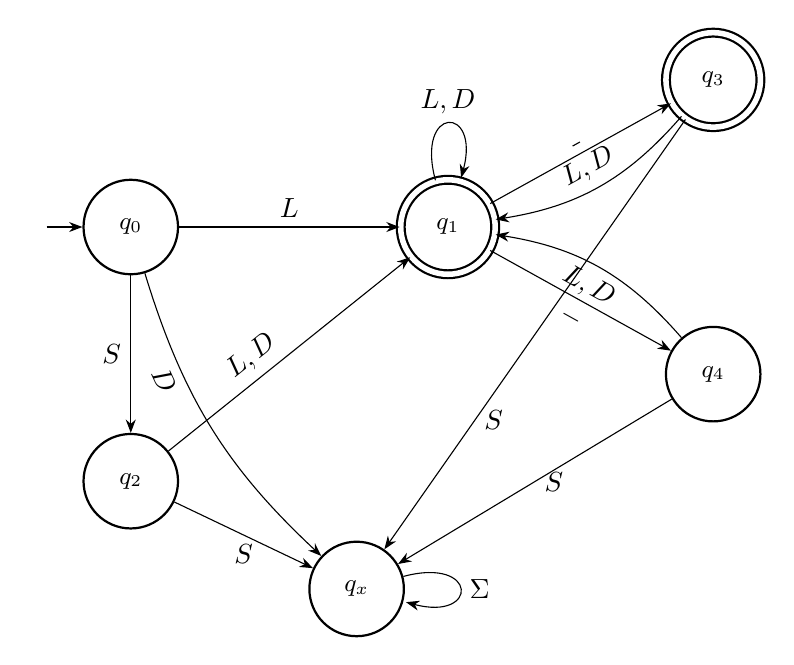
\begin{tikzpicture}[
    ->,
    >=Stealth,
    node distance=2.8cm,
    every state/.style={thick, minimum size=12mm, font=\small},
    accepting/.style={double distance=2pt}
]
    \node[state, initial, initial text=] (q0) {$q_0$};
    \node[state, accepting, right=of q0] (q1) {$q_1$};
    \node[state, below=2cm of q0] (q2) {$q_2$};
    \node[state, accepting, above right=1cm and 2.5cm of q1] (q3) {$q_3$};
    \node[state, below right=1cm and 2.5cm of q1] (q4) {$q_4$};
    \node[state, below right=0.5cm and 2cm of q2] (qx) {$q_x$};

    \path (q0) edge node[above] {$L$} (q1);
    \path (q0) edge node[left] {$S$} (q2);
    \path (q0) edge[bend right=15] node[below,sloped,pos=0.3] {$D$} (qx);

    \path (q1) edge[loop above] node {$L, D$} (q1);
    \path (q1) edge node[above,sloped] {$\_$} (q3);
    \path (q1) edge node[below,sloped] {$-$} (q4);

    \path (q2) edge node[above,sloped,pos=0.4] {$L, D$} (q1);
    \path (q2) edge node[below] {$S$} (qx);

    \path (q3) edge[bend left=20] node[above,sloped] {$L, D$} (q1);
    \path (q3) edge node[right,pos=0.7] {$S$} (qx);

    \path (q4) edge[bend right=20] node[below,sloped] {$L, D$} (q1);
    \path (q4) edge node[right] {$S$} (qx);

    \path (qx) edge[loop right] node {$\Sigma$} (qx);
\end{tikzpicture}
\end{center}

Double circles indicate accepting states. The arrow pointing to \(q_0\) marks it as the start state.

\textbf{Wait, This is Already a DFA}?

Look at what we built. From each state, each input symbol leads to exactly one next state. There are no \(\varepsilon\)-transitions. There is no nondeterminism.

This is already a DFA. By thinking carefully about what information to track, we derived a deterministic automaton directly. No subset construction needed.

This happens more often than you might expect. Many practical patterns lead to automata where the ``obvious'' states are already deterministic. The subset construction is necessary in the general case, but for hand-designed automata targeting specific patterns, you can often avoid it.

\subsection{Transition Table}

For implementation, we need the transition function in table form. This table tells us: given a current state and an input character, what is the next state?

\begin{table}[h]
\centering
\begin{tabular}{c|cccc}
\toprule
& $L$ & $D$ & $\_$ & $-$ \\
\midrule
$q_0$ & $q_1$ & $q_x$ & $q_2$ & $q_2$ \\
$q_1$ & $q_1$ & $q_1$ & $q_3$ & $q_4$ \\
$q_2$ & $q_1$ & $q_1$ & $q_x$ & $q_x$ \\
$q_3$ & $q_1$ & $q_1$ & $q_x$ & $q_x$ \\
$q_4$ & $q_1$ & $q_1$ & $q_x$ & $q_x$ \\
$q_x$ & $q_x$ & $q_x$ & $q_x$ & $q_x$ \\
\bottomrule
\end{tabular}
\caption{Transition function \(\delta(q, c)\). Characters not in \(\Sigma\) lead to \(q_x\).}
\end{table}


Let us trace through a few strings to verify our automaton works correctly.

For \texttt{my\_var}, which should be accepted:
\[
q_0 \xrightarrow{\texttt{m}} q_1 \xrightarrow{\texttt{y}} q_1 \xrightarrow{\texttt{\_}} q_3 \xrightarrow{\texttt{v}} q_1 \xrightarrow{\texttt{a}} q_1 \xrightarrow{\texttt{r}} q_1
\]
Final state \(q_1\) is accepting.

For \texttt{\_init}, which should be accepted:
\[
q_0 \xrightarrow{\texttt{\_}} q_2 \xrightarrow{\texttt{i}} q_1 \xrightarrow{\texttt{n}} q_1 \xrightarrow{\texttt{i}} q_1 \xrightarrow{\texttt{t}} q_1
\]
Final state \(q_1\) is accepting.

For \texttt{a\_\_b}, which should be rejected:
\[
q_0 \xrightarrow{\texttt{a}} q_1 \xrightarrow{\texttt{\_}} q_3 \xrightarrow{\texttt{\_}} q_x
\]
Consecutive symbols lead to the trap state.

For \texttt{test-}, which should be rejected:
\[
q_0 \xrightarrow{\texttt{t}} q_1 \xrightarrow{\texttt{e}} q_1 \xrightarrow{\texttt{s}} q_1 \xrightarrow{\texttt{t}} q_1 \xrightarrow{\texttt{-}} q_4
\]
Final state \(q_4\) is not accepting.

% =============================================================================
\section{Turning It Into Code}
% =============================================================================

With the automaton designed, implementation is straightforward. We precompute the transition table at initialization time, then validation becomes a simple loop.

\subsection{Representing States}

\begin{lstlisting}[language=Go]
const (
    numState = 6

    q0 = iota // start
    q1        // last char was letter/digit
    q2        // started with symbol, need alphanumeric
    q3        // last char was underscore
    q4        // last char was hyphen
    qx        // trap
)
\end{lstlisting}

\subsection{Building the Transition Table}

Recall that a DFA is defined by its transition function \(\delta : Q \times \Sigma \to Q\). Given a state and an input symbol, \(\delta\) tells us the next state. In our theoretical treatment, we wrote this as a table with rows for states and columns for character classes (\(L\), \(D\), \(\_\), \(-\)).

In code, we represent \(\delta\) as a two-dimensional array:

\begin{lstlisting}[language=Go]
var dfa [numState][256]uint8
\end{lstlisting}

The lookup \texttt{dfa[q][c]} gives us \(\delta(q, c)\), the next state when we are in state \texttt{q} and read character \texttt{c}.

Why 256? A byte can hold values from 0 to 255. By making the second dimension 256, we can use any byte value directly as an index. No mapping function, no bounds checking, just \texttt{dfa[state][c]}. This is as fast as array indexing gets.

Our actual alphabet is much smaller: 52 letters, 10 digits, and 2 symbols. We could use a 64-entry table with a mapping function that converts characters to indices. But that mapping function would run on every character. For a hot path, eliminating that overhead matters.

The cost is memory: \(6 \times 256 = 1536\) bytes. This is small enough to fit in L1 cache on any modern processor. The trade-off is clearly in favor of the larger table.

What about characters outside our alphabet? They also need a destination state. We set them to \(q_x\), the trap state. This happens automatically because we initialize every entry to \(q_x\) before filling in the valid transitions.

\begin{lstlisting}[language=Go]
var (
    accepted uint8
    dfa      [numState][256]uint8
)

func init() {
    accepted = (1 << q1) | (1 << q3)
    for q := range numState {
        for b := range 256 {
            c := byte(b)
            dfa[q][b] = qx 
            switch q {
            case q0:
                if isLetter(c) {
                    dfa[q][b] = q1
                } else if c == '_' || c == '-' {
                    dfa[q][b] = q2
                }
            case q1:
                if isLetter(c) || isDigit(c) {
                    dfa[q][b] = q1
                } else if c == '_' {
                    dfa[q][b] = q3
                } else if c == '-' {
                    dfa[q][b] = q4
                }
            case q2, q3, q4:
                if isLetter(c) || isDigit(c) {
                    dfa[q][b] = q1
                }
            }
        }
    }
}
\end{lstlisting}

The initialization loop fills in the transition table at program startup. For each state \texttt{q} and each possible byte value \texttt{b}, we determine the next state based on what character \texttt{c} represents. This matches our theoretical transition table exactly, just expanded to cover all 256 byte values instead of just the four character classes.

The variable \texttt{accepted} is a bitmask that encodes which states are accepting. Bit 1 corresponds to \(q_1\), bit 3 corresponds to \(q_3\). We set both because those are our accepting states.

\subsection{Validator}

The validation function implements the DFA execution algorithm. Start in the initial state. Read characters one by one. For each character, look up the next state in the transition table. After reading all characters, check if the final state is accepting.

\begin{lstlisting}[language=Go]
func Valid(s string) bool {
    if len(s) == 0 {
        return false
    }
    state := uint8(q0)
    for _, c := range s {
        state = dfa[state][c]
        if state == qx {
            return false
        }
    }
    return (accepted >> state) & 1 != 0
}
\end{lstlisting}

The core of the function is the loop. Each iteration does one table lookup: \texttt{state = dfa[state][c]}. This is \(\delta\) in action. We update the state based on the current state and the current character.

We check for the trap state inside the loop. Once we enter \(q_x\), we can never leave it, and we can never reach an accepting state. So we exit early. This is an optimization for invalid inputs.

The final line checks acceptance. The expression \texttt{(accepted >> state) \& 1} extracts bit \texttt{state} from the bitmask. If that bit is 1, the state is accepting and we return true.

Empty strings are rejected upfront. Our DFA requires at least one character to reach any accepting state, so an empty string can never be valid.

\subsection{Character Classification}

\begin{lstlisting}[language=Go]
func isLetter(c byte) bool {
    return (c >= 'a' && c <= 'z') || (c >= 'A' && c <= 'Z')
}

func isDigit(c byte) bool {
    return c >= '0' && c <= '9'
}
\end{lstlisting}

% =============================================================================
\section{How Fast Is It?}
% =============================================================================

\subsection{Time and Space}

The DFA approach gives us \(O(n)\) time where \(n\) is the string length. Each character requires one array lookup. Space at runtime is \(O(1)\). The transition table is 1536 bytes, allocated once at startup. There are zero heap allocations during validation.

\subsection{Benchmarks}

The following benchmarks were run on an Apple M1 Pro (darwin/arm64) using Go's testing framework with \texttt{benchstat} for statistical analysis. Each benchmark was run 10 times.

\begin{table}[h]
\centering
\small
\begin{tabular}{lrrr}
\toprule
\textbf{Benchmark} & \textbf{regexp (ns/op)} & \textbf{DFA (ns/op)} & \textbf{Improvement} \\
\midrule
short\_valid & 102.2 & 3.3 & -96.75\% \\
short\_invalid & 42.8 & 1.3 & -97.06\% \\
medium\_valid & 323.5 & 22.9 & -92.91\% \\
medium\_invalid & 142.4 & 4.0 & -97.16\% \\
long\_valid & 740.9 & 79.2 & -89.32\% \\
long\_invalid & 2026.5 & 75.5 & -96.28\% \\
complex\_valid & 469.7 & 48.9 & -89.59\% \\
complex\_invalid & 439.5 & 10.9 & -97.52\% \\
\midrule
\textbf{geomean} & 298.2 & 13.7 & \textbf{-95.41\%} \\
\bottomrule
\end{tabular}
\caption{Benchmark comparison between regexp and DFA implementations.}
\end{table}

The DFA implementation is roughly 10 to 30 times faster depending on the input. Invalid inputs that fail early in the DFA show the largest improvements because they hit the trap state and exit immediately.

These numbers look impressive, but benchmarks should be interpreted with care.

Microbenchmarks are not real workloads. In a real application, validation is rarely the bottleneck. I/O, network latency, and database queries typically dominate.

Results vary by hardware. The M1 Pro has excellent branch prediction and cache performance. Results on other architectures may differ.

Go's regexp is not slow. It uses RE2, which guarantees linear time. The overhead comes from the general-purpose machinery that handles arbitrary patterns.

Nanoseconds matter only at scale. If you validate 100 strings per request, saving 300ns each gives you 30\textmu s. Probably not worth the added complexity.

The DFA approach makes sense when validation is genuinely on the hot path: parsing millions of log lines, validating every field in a high-throughput data pipeline, or implementing a lexer. For most applications, the standard \texttt{regexp} package is fine.

% =============================================================================
\section{Wrapping Up}
% =============================================================================

We started with a validation problem and ended with a fast, allocation-free implementation.

The process was straightforward. Formalize the problem by writing out the regular expression. This forces you to think precisely about edge cases. Identify states by asking what information you need to remember as you scan the string. Build the transition table, draw the diagram, trace through examples. Then implement. With a clear specification, the code almost writes itself.

This approach is not always necessary. For one-off validations or complex patterns, regex is fine. But when validation is on the critical path and runs millions of times, a custom DFA is worth considering.

More than the specific technique, I hope this paper illustrates a broader point. Fundamentals matter. Automata theory might seem academic and disconnected from day-to-day programming. But when you hit the limits of general-purpose tools, that theoretical foundation becomes practical. It gives you the vocabulary to think about the problem and the tools to solve it.

Do not skip the fundamentals. They are not just for passing exams. They are for moments when you need to build something that does not exist yet.

The complete implementation is available at: \url{https://github.com/josestg/dfaregexp}

\end{document}
